\providecommand{\setflag}{\newif \ifwhole \wholefalse}
\setflag
\ifwhole\else

% Typography and geometry ----------------------------------------------------
\documentclass[letterpaper]{scrbook}
\usepackage[inner=3cm,top=2.5cm,outer=3.5cm]{geometry}

\renewcommand\familydefault{bch}
\usepackage[utf8]{inputenc}
\usepackage{microtype}
\usepackage[small]{caption}
\usepackage[small]{titlesec}
\raggedbottom

% Graphics -------------------------------------------------------------------
\usepackage[pdftex]{graphicx}
\graphicspath{{_include/}}
\DeclareGraphicsExtensions{.png,.pdf}

% Code formatting ------------------------------------------------------------
\usepackage{fancyvrb}
\usepackage{courier}
\usepackage{listings}
\usepackage{color}
\usepackage{alltt}


\definecolor{comment}{rgb}{0.60, 0.60, 0.53}
\definecolor{background}{rgb}{0.97, 0.97, 1.00}
\definecolor{string}{rgb}{0.863, 0.066, 0.266}
\definecolor{number}{rgb}{0.0, 0.6, 0.6}
\definecolor{variable}{rgb}{0.00, 0.52, 0.70}
\lstset{
  basicstyle=\ttfamily,
  keywordstyle=\bfseries, 
  identifierstyle=,  
  commentstyle=\color{comment} \emph,
  stringstyle=\color{string},
  showstringspaces=false,
  columns = fullflexible,
  backgroundcolor=\color{background},
  mathescape = true,
  escapeinside=&&,
  fancyvrb
}
\newcommand{\code}[1]{\lstinline!#1!}
\newcommand{\f}[1]{\lstinline!#1()!}



% Links ----------------------------------------------------------------------

\usepackage{hyperref}
\definecolor{slateblue}{rgb}{0.07,0.07,0.488}
\hypersetup{colorlinks=true,linkcolor=slateblue,anchorcolor=slateblue,citecolor=slateblue,filecolor=slateblue,urlcolor=slateblue,bookmarksnumbered=true,pdfview=FitB}
\usepackage{url}

% Tables ---------------------------------------------------------------------
\usepackage{longtable}
\usepackage{booktabs}

% Miscellaneous --------------------------------------------------------------
\usepackage{pdfsync}
\usepackage{appendix}

\usepackage[round,sort&compress,sectionbib]{natbib}
\bibliographystyle{plainnat}


\title{ggplot2}
\author{Hadley Wickham}

\begin{document}
\fi


% SET_DEFAULTS
%   GG-WIDTH: 4  GG-HEIGHT: 4
%   TEX-WIDTH: 0.5\linewidth
%   CACHE: TRUE
%   INLINE: FALSE
% 
% options(digits = 2, width = 60)

% END

\chapter{Manipulating data}
\label{cha:data}

So far this book has assumed you have your data in a nicely structured data frame ready to feed to \f{ggplot} or \f{qplot}. If this is not the case, then you'll need to do some transformation.  

In Section~\ref{sec:plyr}, you will learn how to use the \pkg{plyr} package to reproduce the statistical transformations performed by the layers, and then in Section~\ref{sec:melting} you will learn a little about ``molten'' (or long) data, which is useful for time series and parallel coordinates plots, among others.  Section~\ref{sec:methods} shows you how to write methods that let you plot objects other than data frames, and demonstrates how \ggplot can be used to re-create a more flexible version of the built in linear-model diagnostics.  

Data cleaning, manipulation and transformation is a big topic and this chapter only scratches the surface of topics closely related to \ggplot.  I recommend the following references which go into considerably more depth on this topic:

\begin{itemize}
  \item \emph{Data Manipulation with R}, by Phil Spector.  Published by Springer, 2008.
  
  \item ``plyr: divide and conquer for data analysis'', Hadley Wickham.  Available from \url{http://had.co.nz/plyr}.  This is a full description of the package used in Section~\ref{sec:plyr}.

  \item ``Reshaping data with the reshape package'', Hadley Wickham. \emph{Journal of Statistical Software}, 21(12), 2007. \url{http://www.jstatsoft.org/v21/i12/}.  This describes the complement of the melt function used in Section~\ref{sec:melting}, which can be used like pivot tables to create a wide range of data summaries and rearrangements.
  
\end{itemize}

\section{An introduction to plyr}
\label{sec:plyr}

With faceting, \ggplot makes it very easy to create identical plots for different subsets of your data. This section introduces \f{ddply} from the \pkg{plyr} package, a function that makes it easy to do the same thing for numerical summaries. \pkg{plyr} provides a comprehensive suite of tools for breaking up complicated data structures into pieces, processing each piece and then joining the results back together. The \pkg{plyr} package as a whole provides tools for breaking and combining lists, arrays and data frames. Here we will focus on the \f{ddply} function which breaks up a data frame into subsets based on row values, applies a function to each subset and then joins the results back into a data frame. The basic syntax is \code{ddply(.data, .variables, .fun, ...)}, where

\begin{itemize}

  \item \code{.data} is the dataset to break up (e.g., the data that you are plotting).

  \item \code{.variables} is a description of the grouping variables used to break up the dataset. This is written like \code{.(var1, var2)}, and to match the plot should contain all the grouping and faceting variables that you've used in the plot.

  \item \code{.fun} is the summary function you want to use. The function can return a vector or data frame. The result does not need to contain the grouping variables: these will be added on automatically if they're needed. The result can be a much reduced aggregated dataset (maybe even one number), or the original data modified or expanded in some way.

\end{itemize}

More information and examples are available in the documentation, \code{?ddply}, and on the package website, \url{http://had.co.nz/plyr}.  The following examples show a few useful summary functions that solve common data manipulation problems.

\begin{itemize}
  \item Using \f{subset} allows you to select the top (or bottom) n (or x\%) of observations in each group, or observations above (or below) some group-specific threshold:
  
  % LISTING
  % 
  % # Select the smallest diamond in each colour
  % ddply(diamonds, .(color), subset, carat == min(carat))
  % 
  % # Select the two smallest diamonds
  % ddply(diamonds, .(color), subset, order(carat) < 2)
  % 
  % # Select the 1% largest diamonds in each group
  % ddply(diamonds, .(color), subset, carat > quantile(carat, 0.99))
  % 
  % # Select all diamonds bigger than the group average
  % ddply(diamonds, .(color), subset, price > mean(price))
  \input{_include/cafc08f2d0bf1d229a8ca8fce823a80f.tex}  
  % END
  
  \item Using \f{transform} allows you to perform group-wise transformations with very little work.  This is particularly useful if you want to add new variables that are calculated on a per-group level, such as a per-group standardisation.  Section~\ref{sub:time-series} shows another use of this technique for standardising time series to a common scale.
  
  % LISTING
  % 
  % # Within each colour, scale price to have mean 0 and variance 1
  % ddply(diamonds, .(color), transform, price = scale(price))
  % 
  % # Subtract off group mean
  % ddply(diamonds, .(color), transform, price = price - mean(price))
  \input{_include/a96f045aa9ce7a20784582ad5e08258e.tex}  
  % END

  \item If you want to apply a function to every column in the data frame, you might find the \f{colwise} function handy. This function converts a function that operates on vectors to a function that operates column-wise on data frames. This is rather different than most functions: instead of returning a vector of numbers, \f{colwise} returns a new function. The following example creates a function to count the number of missing values in a vector and then shows how we can use \f{colwise} to apply it to every column in a data frame.

  % INTERWEAVE
  % 
  % nmissing <- function(x) sum(is.na(x))
  % nmissing(msleep$name)
  % nmissing(msleep$brainwt)
  % 
  % nmissing_df <- colwise(nmissing)
  % nmissing_df(msleep)
  % # This is shorthand for the previous two steps
  % colwise(nmissing)(msleep)
  \input{_include/9d12f4c4140cfb43f030ee92bc3ed8f0.tex}  
  % END
  
   The specialised version \f{numcolwise} does the same thing, but works only with numeric columns.  For example, \code{numcolwise(median)} will calculate a median for every numeric column, or \code{numcolwise(quantile)} will calculate quantiles for every numeric column.  Similarly, \f{catcolwise} only works with categorical columns.
  
  % INTERWEAVE
  % 
  % msleep2 <- msleep[, -6] # Remove a column to save space
  % numcolwise(median)(msleep2, na.rm = T)
  % numcolwise(quantile)(msleep2, na.rm = T)
  % numcolwise(quantile)(msleep2, probs = c(0.25, 0.75), na.rm = T)
  \input{_include/22973fb980c0459fe3face8a29226149.tex}  
  % END
  
  Combined with \code{ddply}, this makes it easy to produce per-group summaries:
  
  % INTERWEAVE
  % 
  % ddply(msleep2, .(vore), numcolwise(median), na.rm = T)
  % ddply(msleep2, .(vore), numcolwise(mean), na.rm = T)
  \input{_include/77ecfb1a6bdeb2bdfcd51f50d5635dd2.tex}  
  % END
  
  \item If none of the previous shortcuts is appropriate, make your own summary function which takes a data frame as input and returns an appropriately summarised data frame as output.  The following function calculates the rank correlation of price and carat and compares it to the regular correlation of the logged values.
  
  % INTERWEAVE
  % 
  % my_summary <- function(df) {
  %   with(df, data.frame(
  %     pc_cor = cor(price, carat, method = "spearman"),
  %     lpc_cor = cor(log(price), log(carat))
  %   ))
  % }
  % ddply(diamonds, .(cut), my_summary)
  % ddply(diamonds, .(color), my_summary)
  \input{_include/0d97442ce4527f151003d26ae6153bde.tex}  
  % END
  
  Note how our summary function did not need to output the group variables.  This makes it much easier to aggregate over different groups.
\end{itemize}

The common pattern of all these problems is that they are easy to solve if we have the right subset. Often the solution for a single case might be a single line of code. The difficulty comes when we want to apply the function to multiple subsets and then correctly join back up the results. This may take a lot of code, especially if you want to preserve group labels. \f{ddply} takes care of all this for you.

The following case study shows how you can use \pkg{plyr} to reproduce the statistical summaries produced by \ggplot.  This is useful if you want to save them to disk or apply them to other datasets.  It's also useful to be able to check that \ggplot is doing exactly what you think!

\subsection{Fitting multiple models}
\label{sub:multiple_models}

In this section, we'll work through the process of generating the smoothed data produced by \code{stat_smooth}.  This process will be the same for any other statistic, and should allow you to produce more complex summaries that \ggplot can't produce by itself.  Figure~\ref{fig:smooth} shows the group-wise smoothes produced by the following code.

% FIGLISTING
%   LABEL: smooth
%   CAPTION: A plot showing the smoothed trends for price vs. carat for each
%   colour of diamonds.  With the full range of carats (left), the standard
%   errors balloon after around two carats because there are relatively few
%   diamonds of that size.  Restricting attention to diamonds of less than
%   two carats (right) focuses on the region where we have plenty of data.
% 
% qplot(carat, price, data = diamonds, geom = "smooth", colour = color)
% dense <- subset(diamonds, carat < 2)
% qplot(carat, price, data = dense, geom = "smooth", colour = color, 
%   fullrange = TRUE)
\input{_include/520432aa266eedd0a71583c6140ae9a8.tex}
% END

How can we re-create this by hand?  First we read the \f{stat_smooth} documentation to determine what the model is: for large data it's \code{gam(y ~ s(x, bs = "cs"))}.  To get the same output as \f{stat_smooth}, we need to fit the model, then predict it on an evenly spaced grid of points. This task is performed by the \f{smooth} function in the following code.  Once we have written this function it is straightforward to apply it to each diamond colour  using \f{ddply}.

Figure~\ref{fig:smooth-by-hand} shows the results of this work, which are identical to what we got with \ggplot doing all the work.

% FIGLISTING
%   LABEL: smooth-by-hand
%   CAPTION: Figure~\ref{fig:smooth} with all statistical calculations 
%   performed by hand.  The predicted values (left), and with standard errors
%   (right).
% 
% library(mgcv)
% smooth <- function(df) {
%   mod <- gam(price ~ s(carat, bs = "cs"), data = df)
%   grid <- data.frame(carat = seq(0.2, 2, length = 50))
%   pred <- predict(mod, grid, se = T)
%   
%   grid$price <- pred$fit
%   grid$se <- pred$se.fit
%   grid
% }
% smoothes <- ddply(dense, .(color), smooth)
% qplot(carat, price, data = smoothes, colour = color, geom = "line")
% qplot(carat, price, data = smoothes, colour = color, geom = "smooth",
%   ymax = price + 2 * se, ymin = price - 2 * se)
\input{_include/a95443c42067de3ec12c6760b2752feb.tex}
% END

Doing the summary by hand gives you much more flexibility to fit models where the grouping factor is explicitly included as a covariate. For example, the following model models price as a non-linear function of carat, plus a constant term for each colour. It's not a very good model as it predicts negative prices for small, poor-quality diamonds, but it's a starting point for a better model.

% INTERWEAVE
% 
% mod <- gam(price ~ s(carat, bs = "cs") + color, data = dense)
% grid <- with(diamonds, expand.grid(
%   carat = seq(0.2, 2, length = 50),
%   color = levels(color)
% ))
% grid$pred <- predict(mod, grid)
% qplot(carat, pred, data = grid, colour = color, geom = "line")
\input{_include/bef542d564afa3b3e46830bf2b9c8d03.tex}
% END

See also Sections~\ref{sub:different_aesthetics} and \ref{sec:uncertainty} for other ways of combining models and data.

\section{Converting data from wide to long}
\label{sec:melting}

In \ggplot graphics, groups are defined by rows, not by columns. This makes it easy to draw a line for each group defined by the value of a variable (or set of variables) but difficult to draw a separate line for each variable. In this section you will learn how to transform your data to a form in which you can draw a line for each variable. This transformation converts from ``wide'' data to ``long'' data, where each variable now occupies its own set of rows.

To perform this transformation we will use the \f{melt} function from the \pkg{reshape} package \citep{wickham:2007b}. Reshape also provides the \f{cast} function to flexibly reshape and aggregate data, which you may want to read about yourself. Table~\ref{tbl:melt} gives an example. The \f{melt} function has three arguments:

\begin{itemize}

  \item \code{data}: the data frame you want to convert to long form.

  \item \code{id.vars}: Identifier (id) variables identify the unit that measurements take place on. Id variables are usually discrete, and are typically fixed by design. In {\sc anova} notation ($Y_{ijk}$), id variables are the indices on the variables ($i, j, k$); in database notation, id variables are a composite primary key.

  \item \code{measure.vars}: Measured variables represent what is measured on that unit ($Y$). These will be the variables that you want to display simultaneously on the plot.

\end{itemize}

If you're familiar with Wilkinson's grammar of graphics, you might wonder why there is no equivalent to the algebra.  There is no equivalent to the algebra within \ggplot itself because there are many other facilities for transforming data in R, and it is in line with the \ggplot philosophy of keeping data transformation and visualisation as separate as possible.

% library(xtable)
% xtable(format(head(economics), digits = 2)[, 1:3])
% em <- melt(head(economics), id = "date", m = c("pce", "pop"))
% xtable(format(em, digits = 2))

\begin{table}[ht]
  \centering
  \begin{minipage}[t]{0.4\linewidth}
  \begin{tabular}{rrr}
    \toprule
    date & pce & pop \\
    \midrule
    1967-06-30 & 508 & 198,712 \\
    1967-07-31 & 511 & 198,911 \\
    1967-08-31 & 517 & 199,113 \\
    1967-09-30 & 513 & 199,311 \\
    1967-10-31 & 518 & 199,498 \\
    1967-11-30 & 526 & 199,657 \\
    \bottomrule
  \end{tabular}
  \end{minipage}
  \hspace{0.5cm}
  \begin{minipage}[t]{0.4\linewidth}
  \begin{tabular}{rrr}
    \toprule
    date & variable & value \\
    \midrule
    1967-06-30 & pce &     508 \\
    1967-07-31 & pce &     511 \\
    1967-08-31 & pce &     517 \\
    1967-09-30 & pce &     513 \\
    1967-10-31 & pce &     518 \\
    1967-11-30 & pce &     526 \\
    1967-06-30 & pop & 198,712 \\
    1967-07-31 & pop & 198,911 \\
    1967-08-31 & pop & 199,113 \\
    1967-09-30 & pop & 199,311 \\
    1967-10-31 & pop & 199,498 \\
    1967-11-30 & pop & 199,657 \\
    \midrule
  \end{tabular}
  \end{minipage}

  \caption{Economics data in wide, left, and long, right, formats.  The data stored in each table is equivalent, just the arrangement is different.  It it easy to use the wider format with \ggplot to produce a line for each variable.}
  \label{tbl:melt}
\end{table}

The following sections explore two important uses of molten data in more detail: plotting multiple time series and creating parallel coordinate plots. You will also see how to use \f{ddply} to rescale the variables, and learn about the features of \ggplot that are most useful in conjunction with this sort of data.

\subsection{Multiple time series}
\label{sub:time-series}

Take the \code{economics} dataset.  It contains information about monthly economic data like the number of people unemployed (\code{unemploy}) and the median length of unemployment (\code{uempmed}).  We might expect these two variables to be related.  Each of these variables is stored in a column, which makes it easy to compare them with a scatterplot, and draw individual time series, as shown in Figure~\ref{fig:series-wide}.  But what if we want to see the time series them simultaneously?

% FIGURE
%   COL: 3  TEX-WIDTH: 0.33\linewidth
%   LABEL: series-wide
%   CAPTION: When the economics dataset is stored in wide format, it is easy
%   to create separate time series plots for each variable (left and centre),
%   and easy to create scatterplots comparing them (right).
% 
% qplot(date, uempmed, data = economics, geom = "line")
% qplot(date, unemploy, data = economics, geom = "line")
% qplot(unemploy, uempmed, data = economics) + geom_smooth()
\input{_include/f10d7186458002334b71daac504495c3.tex}
% END

One way is to build up the plot with a different layer for each variable, as you saw in Section~\ref{sub:scale-manual}. However, this quickly becomes tedious when you have many variables, and a better alternative is to melt the data into a long format and then visualise that. In the molten data the time series have their value stored in the \var{value} variable and we can distinguish between them with the \var{variable} variable. The code below shows these two alternatives. The plots they produce are very similar, and are shown in Figure~\ref{fig:series-methods}.

% FIGLISTING
%   LABEL: series-methods GG-HEIGHT: 3 GG-WIDTH: 6
%   CAPTION: The two methods of displaying both series on a single plot 
%   produce identical plots, but using long data is much easier when you have
%   many variables.  The series have radically different scales, so we only
%   see the pattern in the \code{unemploy} variable. You might not even notice
%   \code{uempmed} unless you're paying close attention: it's the line at the
%   bottom of the plot.
% 
% ggplot(economics, aes(date)) + 
%   geom_line(aes(y = unemploy, colour = "unemploy")) + 
%   geom_line(aes(y = uempmed, colour = "uempmed")) + 
%   scale_colour_hue("variable")
%
% emp <- melt(economics, id = "date", measure = c("unemploy", "uempmed"))
% qplot(date, value, data = emp, geom = "line", colour = variable)
\input{_include/1656d12f67fd9113f430fd635d40b9da.tex}
% END

There is a problem with these plots: the two variables have radically different scales, and so the series for \code{uempmed} appears as a flat line at the bottom of the plot. There is no way to produce a plot with two axes in \ggplot because this type of plot is fundamentally misleading. Instead there are two perceptually well-founded alternatives: rescale the variables to have a common range, or use faceting with free scales. These alternatives are created with the code below and are shown in Figure~\ref{fig:series-scaling}

% FIGLISTING
%   LABEL: series-scaling 
%   GG-HEIGHT: 3 GG-WIDTH: 6
%   CAPTION: When the series have very different scales we have two 
%   alternatives: left, rescale the variables to a common scale, or right,
%   display the variables on separate facets and using free scales.
% 
% range01 <- function(x) {
%   rng <- range(x, na.rm = TRUE)
%   (x - rng[1]) / diff(rng)
% }
% emp2 <- ddply(emp, .(variable), transform, value = range01(value))
% qplot(date, value, data = emp2, geom = "line", 
%   colour = variable, linetype = variable)
% qplot(date, value, data = emp, geom = "line") + 
%   facet_grid(variable ~ ., scales = "free_y")
\input{_include/ae989935a36c1578d8372a0660ee3416.tex}
% END

\subsection{Parallel coordinates plot} 
\label{sub:molten_data}

In a similar manner, we can use molten data to create a parallel coordinates plot \citep{inselberg:1985,wegman:1990}, which has the ``variable'' variable on the x axis and value on the y axis.  We need a new variable to record the row that each observation came from, which is used as a grouping variable for the lines (so we get one line per observation). The easiest value to use for this is the data frame \code{rownames}, and we give it an unusual name {\code{.row}, so we don't squash any of the existing variables. Once we have the data in this form, creating a parallel coordinates plot is easy.

The following code does exactly that for the ratings of 840 movies with over 10,000 votes. This dataset has a moderate number of variables (10) and many cases, and will allow us to experiment with a common technique for dealing with large data in parallel coordinates plots: transparency and clustering. Each variable gives the proportion of votes given to each rating between 0 (very bad) and 10 (very good). Since this data is already on a common scale we don't need to rescale it, but in general, we would need to use the technique from the previous section to ensure the variables are comparable. This is particularly important if we are going to use other multidimensional techniques to analyse the data.

% CODELISTING
% 
% popular <- subset(movies, votes > 1e4)
% ratings <- popular[, 7:16]
% ratings$.row <- rownames(ratings)
% molten <- melt(ratings, id = ".row")
\input{_include/db4b6ffbd858aee2875242d855033771.tex}
% END

Once the data is in this form, creating a parallel coordinates plot is easy. All we need is a line plot with \code{variable} on the x axis, \code{value} on the y axis and the lines grouped by \code{.row}. This data needs a few tweaks to the default because the values are highly discrete. In the following code, we experiment with jittering and alpha blending to better display where the bulk of the movies lie. The results are shown in Figure~\ref{fig:pcp}. Most are rated as sevens or eights by around 25\% of voters, with a few exceptional movies getting 35\% of more perfect 10s. However, the large number of lines makes it difficult to distinguish individual movies and it's hard to draw firm conclusions.

% FIGLISTING
%   LABEL: pcp
%   FILETYPE: png GG-WIDTH: 6 COL: 2
%   CAPTION: Variants on the parallel coordinates plot to better display the 
%   patterns in this highly discrete data.  To improve the default pcp
%   (top left) we experiment with alpha blending (top right), jittering 
%   (bottom left) and then both together (bottom right).
%
% pcp <- ggplot(molten, aes(variable, value, group = .row))
% pcp + geom_line()
% pcp + geom_line(colour = alpha("black", 1 / 20))
% jit <- position_jitter(width = 0.25, height = 2.5)
% pcp + geom_line(position = jit)
% pcp + geom_line(colour = alpha("black", 1 / 20), position = jit)
\input{_include/7b8d68c1672208ff82a29b83cd42c430.tex}
% END

To make the patterns more clear we will cluster the movies into groups of similar rating patterns. The following code uses kmeans clustering \citep{hartigan:1979} to produce six groups of similar movies.  To make the clusters a little more interpretable, they are relabelled so that cluster 1 has the lowest average rating and cluster six the highest.

% CODELISTING
% 
% cl <- kmeans(ratings[1:10], 6)
% ratings$cluster <- reorder(factor(cl$cluster), popular$rating)
% levels(ratings$cluster) <- seq_along(levels(ratings$cluster))
% molten <- melt(ratings, id = c(".row", "cluster"))
\input{_include/63b74bfd6718e41ee9b01140f371f2b8.tex}
% END

There are many different ways that we can visualise the result of this clustering. One popular method is shown in Figure~\ref{fig:pcp-colour} where line colour is mapped to group membership. This plot is supplemented with a plot that just shows averages for each group. These plots are both straightforward to create, as shown in the following code.

% FIGLISTING
%   LABEL: pcp-colour
%   FILETYPE: png
%   GG-HEIGHT: 3
%   CAPTION: Displaying cluster membership on a parallel coordinates plot.
%   (Left) Individual movies coloured by group membership and (right) 
%   group means.
% 
% pcp_cl <- ggplot(molten, 
%  aes(variable, value, group = .row, colour = cluster)) 
% pcp_cl + geom_line(position = jit, alpha = 1/5)
% pcp_cl + stat_summary(aes(group = cluster), fun.y = mean, geom = "line")
\input{_include/ea542edf4e62c785101a8cd211167739.tex}
% END

These plots are good for showing the differences between groups, but they don't tell us a lot about whether we've done a good job clustering the data.  Figure~\ref{fig:pcp-facet} uses faceting to display each group in its own panel. This plot highlights the variation within many of the groups, suggesting that perhaps more clusters would be appropriate.

% FIGLISTING
%   LABEL: pcp-facet
%   FILETYPE: png
%   TEX-WIDTH: \linewidth GG-WIDTH: 6
%   CAPTION: Faceting allows us to display each group in its own panel, 
%   highlighting the fact that there seems to be considerable variation
%   within each group, and suggesting that we need more groups in our
%   clustering.
% 
% pcp_cl + geom_line(position = jit, colour = alpha("black", 1/5)) +
%   facet_wrap(~ cluster)
\input{_include/f9b4e59093021f49174f0c9ea45da8f8.tex}
% END


\section{\f{ggplot} methods}
\label{sec:methods}

\f{ggplot} is a generic function, with different methods for different types of data. The most common input, and what we have used until now, is a data frame. As with base and lattice graphics, it is possible to extend \f{ggplot} to work with other types of data. However, the way this works with \ggplot is fundamentally different: \ggplot will not give you a complete plot, but instead will give you the tools you need to make any plot you desire.

This process is mediated by the \f{fortify} method, which takes an object, and optional data frame, and creates a version of the object in a form suitable for plotting with \ggplot, i.e., as a data frame. The name fortify comes from thinking about combining a model with its data: the model fortifies the data, and the data fortifies the model, and the result can be used to simultaneously visualise the model and the data. An example will make this concrete, as you will see when we describe the fortify method for linear models.

This section describes how the \f{fortify} method works, and how you can create new methods that are aligned with the \ggplot philosophy.  The most important philosophical consideration is that data transformation and display should be kept as separate as possible.  This maximises reusability, as you are no longer trapped into the single display that the author envisaged.  

These different types of input also work with \f{qplot}: remember that \f{qplot} is just a thin wrapper around \f{ggplot}.

\subsection{Linear models}

Currently, \ggplot provides only one fortify method, for linear models. Here we'll show how this method works, and how you can use it to create tailored plots for better understanding your data and models. Figure~\ref{fig:plot-lm} shows the output of \f{plot.lm} for a simple model. The graphics are a set of pre-chosen model summary plots. These are useful for particular problems, but are completely inflexible: there is no way to modify them apart from opening up the source code for \f{plot.lm} and modifying it. This is hard because the data transformation and display are inextricably entangled, making the code difficult to understand.

% mod <- lm(cty ~ displ, data = mpg)
% pdf("data-plot-lm.pdf", width = 8, height = 8)
% par(mfrow = c(2, 2))
% plot.lm(mod)
% dev.off()

\begin{figure}[htbp]
  \centering
  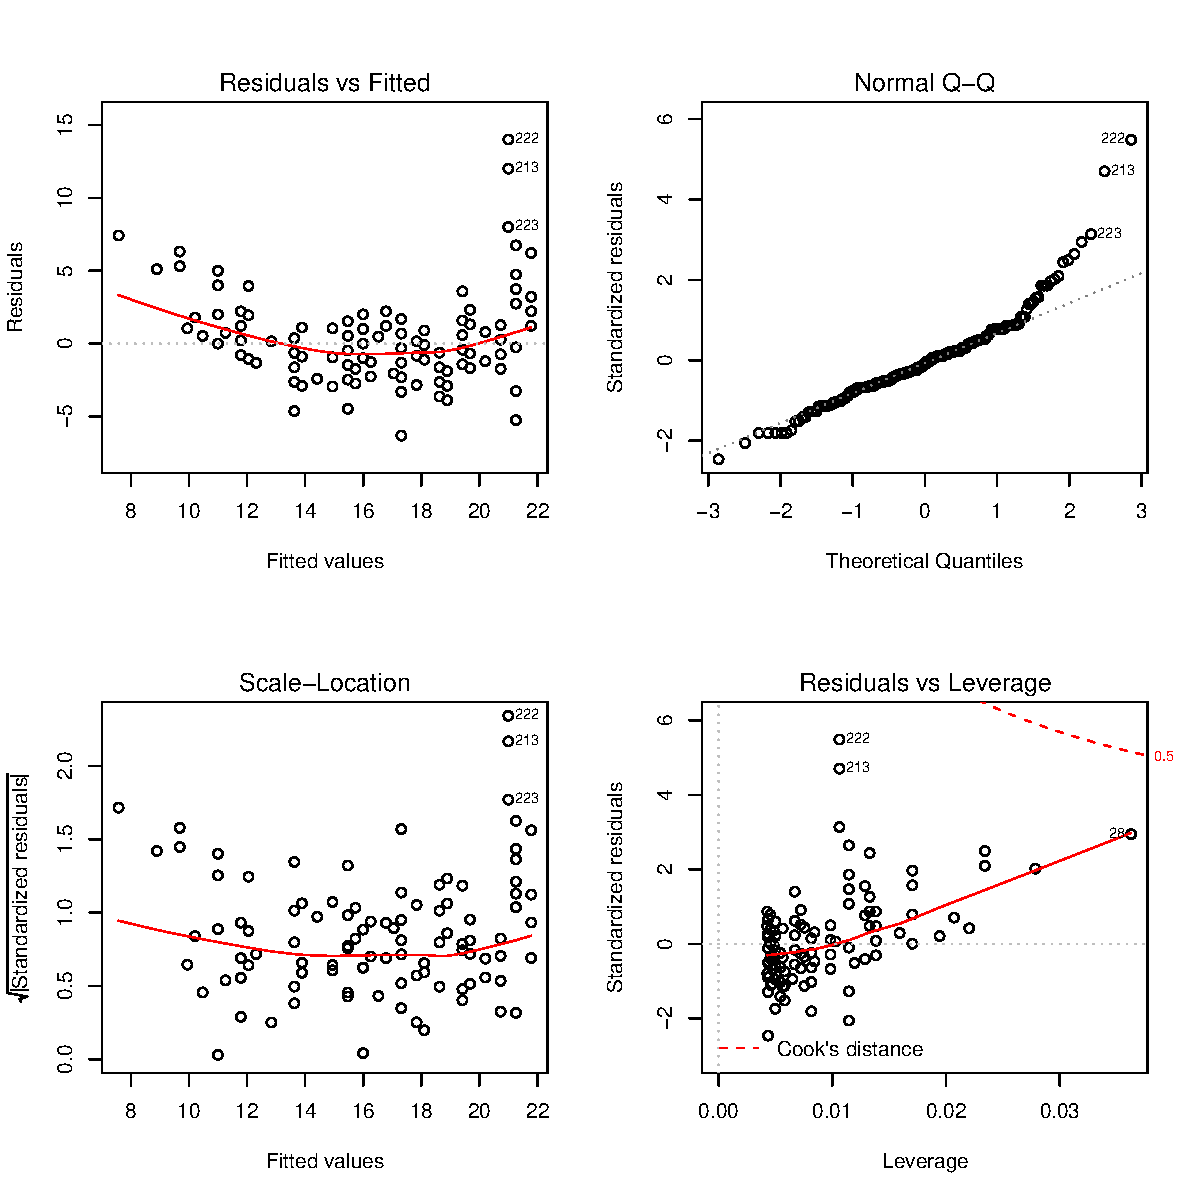
\includegraphics[width=0.8\linewidth]{data-plot-lm}
  \caption{The output from \f{plot.lm} for a simple model.  }
  \label{fig:plot-lm}
\end{figure}

The \ggplot approach completely separates data transformation and display. The \f{fortify} method does the transformation, and then we use \ggplot as usual to create the display that we want. Currently \f{fortify} adds the variables listed in Table~\ref{tbl:fortify-vars} to the original dataset. These are basically all the variables that \f{plot.lm} creates in order to produce its summary plots. The variables have a leading \code{.} (full stop) in their names, so there is little risk that they will clobber variables already in the dataset.

\begin{table}
  \centering
  \begin{tabular}{lp{2.5in}}
    \toprule
    Variable & Description \\
    \midrule
    \code{.cooksd}   & Cook's distances \\
    \code{.fitted}   & Fitted values \\
    \code{.hat}      & Diagonal of the hat matrix \\
    \code{.resid}    & Residuals \\
    \code{.sigma}    & Estimate of residual standard deviation when corresponding observation is dropped from model \\
    \code{.stdresid} & Standardised residuals \\
    \bottomrule
  \end{tabular}
  \caption{The diagnostic variables that \f{fortify.lm} assembles and adds to the model data.}
  \label{tbl:fortify-vars}
\end{table}

% If we just supply \f{fortify} with the model, it will add the diagnostic columns to the model data frame (which just contains the variables used in the model), or we can also supply the full original dataset.  

To demonstrate these techniques, we're going to fit the very simple model with code below, which also creates the plot in Figure~\ref{fig:fortify-mod}. This model clearly doesn't fit the data well, so we should be able to use model diagnostics to figure out how to improve it. A sample of the output from fortifying this model is shown in Table~\ref{tbl:fortify-out}. Because we didn't supply the original data frame, it contains the two variables used in the model as well as the six diagnostic variables. It's easy to see exactly what data our plot will be working with and we could easily add more variables if we wanted.

% FIGLISTING
%   LABEL: fortify-mod
%   CAPTION: A simple linear model that doesn't fit the data very well.
% 
% qplot(displ, cty, data = mpg) + geom_smooth(method = "lm")
% mpgmod <- lm(cty ~ displ, data = mpg)
\input{_include/72863d85cb336f9a6f1348f977e0e401.tex}
% END

% library(xtable)
% xtable(head(fortify(mpgmod)))

\begin{table}[ht]
  \centering
  \begin{tabular}{rrrrrrrrr}
    \toprule
    cty & displ & .hat & .sigma & .cooksd & .fitted & .resid & .stdresid \\
    \midrule
    18 & 1.80 & 0.01 & 2.56 & 0.01 & 21.26 & -3.26 & -1.28 \\
    21 & 1.80 & 0.01 & 2.57 & 0.00 & 21.26 & -0.26 & -0.10 \\
    20 & 2.00 & 0.01 & 2.57 & 0.00 & 20.73 & -0.73 & -0.29 \\
    21 & 2.00 & 0.01 & 2.57 & 0.00 & 20.73 & 0.27 & 0.11 \\
    16 & 2.80 & 0.01 & 2.57 & 0.00 & 18.63 & -2.63 & -1.03 \\
    18 & 2.80 & 0.01 & 2.57 & 0.00 & 18.63 & -0.63 & -0.24 \\
    \bottomrule
  \end{tabular}
  \caption{The output of \code{fortify(mpgmod)} contains the two variables used in the model (\var{cty} and \var{displ}), and the six diagnostic variables described above.}
  \label{tbl:fortify-out}
\end{table}

% You may notice some similarity between this approach and the transformations performed by stats.  The major difference is that \f{fortify} is global, while statistical transformations are local to the facet and group.

With a fortified dataset in hand we can easily re-create the plots produced by \f{plot.lm}, and even better, we can adapt them to our needs. The example below shows how we can re-create and then extend the first plot produced by \f{plot.lm}. Once we have the basic plot we can easily enhance it: use standardised residuals instead of raw residuals, or make size proportional to Cook's distance. The results are shown in Figure~\ref{fig:fortify-fr}.

% FIGLISTING
%   COL: 3 TEX-WIDTH: 0.33\linewidth
%   LABEL: fortify-fr
%   CAPTION: (Left) Basic fitted values-residual plot.  (Middle) With
%   standardised residuals.  (Right) With size proportional to Cook's
%   distance.  It is easy to modify the basic plots when we have access to all
%   of the data.
% 
% mod <- lm(cty ~ displ, data = mpg)
% basic <- ggplot(mod, aes(.fitted, .resid)) +
%   geom_hline(yintercept = 0, colour = "grey50", size = 0.5) + 
%   geom_point() + 
%   geom_smooth(size = 0.5, se = F)
% basic
% basic + aes(y = .stdresid)
% basic + aes(size = .cooksd) + scale_area("Cook's distance")
\input{_include/66a98cfe2e732e16f67dcb00156ac240.tex}
% END

Additionally, we can fortify the whole dataset and add to the plot variables that are in the original data but not in the model. This helps us to understand what variables are useful to improve the model. Figure~\ref{fig:fortify-full} colours the residuals by the number of cylinders, and suggests that this variable would be good to add to the model: within each cylinder group, the pattern is close to linear.

% FIGLISTING
%   LABEL: fortify-full
%   CAPTION: Adding variables from the original data can be enlightening.  
%   Here when we add the number of cylinders we see that instead of a 
%   curvi-linear relationship between displacement and city mpg, it is 
%   essentially linear, conditional on the number of cylinders. 
% 
% full <- basic %+% fortify(mod, mpg)
% full + aes(colour = factor(cyl))
% full + aes(displ, colour = factor(cyl))
\input{_include/1c57abb6c46808b3f1b40a997bad2b02.tex}
% END

\subsection{Writing your own}

To write your own \f{fortify} method, you will need to think about what variables are most useful for model diagnosis, and how they should be returned to the user. The method for linear models adds them on to the original data frame, but this might not be the best approach in other circumstances, and you may instead want to return a list of data frames giving information at different levels of aggregation.

You can also use \f{fortify} with non-model functions.  The following example shows how we could write a \f{fortify} method to make it easier to add images to your plots.  The \pkg{EBImage} from bioconductor is used to get the image into R, and then the fortify method converts it into a form (a data frame) that \ggplot can render.  Should you even need a picture of me on your plot, the following code will allow you to do so.

% LISTING
% 
% fortify.Image <- function(model, data, ...) {
%   colours <- channel(model, "x11")[,,]
%   colours <- colours[, rev(seq_len(ncol(colours)))]
%   melt(colours, c("x", "y"))
% }
% 
% library(EBImage)
% img <- readImage("http://had.co.nz/me.jpeg", TrueColor)
% qplot(x, y, data = img, fill = value, geom="tile") + 
%   scale_fill_identity() + coord_equal()
\input{_include/1316d3d4289e8219eb3253cdd46c03be.tex}
% END

This approach cleanly separates the display of the data from its production, and dramatically improves reuse. However, it does not provide any conveniently pre-packaged functions. If you want to create a diagnostic plot for a linear model you have to assemble all the pieces yourself. Once you have the basic structure in place, so that people can always dig back down and alter the individual pieces, you can write a function that joins all the components together in a useful way. See Section~\ref{sec:functions} for some pointers on how to do this.

\ifwhole
\else
  \nobibliography{/Users/hadley/documents/phd/references}
  \end{document}
\fi
